% Options for packages loaded elsewhere
\PassOptionsToPackage{unicode}{hyperref}
\PassOptionsToPackage{hyphens}{url}
%
\documentclass[
]{article}
\usepackage{amsmath,amssymb}
\usepackage{iftex}
\ifPDFTeX
  \usepackage[T1]{fontenc}
  \usepackage[utf8]{inputenc}
  \usepackage{textcomp} % provide euro and other symbols
\else % if luatex or xetex
  \usepackage{unicode-math} % this also loads fontspec
  \defaultfontfeatures{Scale=MatchLowercase}
  \defaultfontfeatures[\rmfamily]{Ligatures=TeX,Scale=1}
\fi
\usepackage{lmodern}
\ifPDFTeX\else
  % xetex/luatex font selection
\fi
% Use upquote if available, for straight quotes in verbatim environments
\IfFileExists{upquote.sty}{\usepackage{upquote}}{}
\IfFileExists{microtype.sty}{% use microtype if available
  \usepackage[]{microtype}
  \UseMicrotypeSet[protrusion]{basicmath} % disable protrusion for tt fonts
}{}
\makeatletter
\@ifundefined{KOMAClassName}{% if non-KOMA class
  \IfFileExists{parskip.sty}{%
    \usepackage{parskip}
  }{% else
    \setlength{\parindent}{0pt}
    \setlength{\parskip}{6pt plus 2pt minus 1pt}}
}{% if KOMA class
  \KOMAoptions{parskip=half}}
\makeatother
\usepackage{xcolor}
\usepackage[margin=1in]{geometry}
\usepackage{color}
\usepackage{fancyvrb}
\newcommand{\VerbBar}{|}
\newcommand{\VERB}{\Verb[commandchars=\\\{\}]}
\DefineVerbatimEnvironment{Highlighting}{Verbatim}{commandchars=\\\{\}}
% Add ',fontsize=\small' for more characters per line
\usepackage{framed}
\definecolor{shadecolor}{RGB}{248,248,248}
\newenvironment{Shaded}{\begin{snugshade}}{\end{snugshade}}
\newcommand{\AlertTok}[1]{\textcolor[rgb]{0.94,0.16,0.16}{#1}}
\newcommand{\AnnotationTok}[1]{\textcolor[rgb]{0.56,0.35,0.01}{\textbf{\textit{#1}}}}
\newcommand{\AttributeTok}[1]{\textcolor[rgb]{0.13,0.29,0.53}{#1}}
\newcommand{\BaseNTok}[1]{\textcolor[rgb]{0.00,0.00,0.81}{#1}}
\newcommand{\BuiltInTok}[1]{#1}
\newcommand{\CharTok}[1]{\textcolor[rgb]{0.31,0.60,0.02}{#1}}
\newcommand{\CommentTok}[1]{\textcolor[rgb]{0.56,0.35,0.01}{\textit{#1}}}
\newcommand{\CommentVarTok}[1]{\textcolor[rgb]{0.56,0.35,0.01}{\textbf{\textit{#1}}}}
\newcommand{\ConstantTok}[1]{\textcolor[rgb]{0.56,0.35,0.01}{#1}}
\newcommand{\ControlFlowTok}[1]{\textcolor[rgb]{0.13,0.29,0.53}{\textbf{#1}}}
\newcommand{\DataTypeTok}[1]{\textcolor[rgb]{0.13,0.29,0.53}{#1}}
\newcommand{\DecValTok}[1]{\textcolor[rgb]{0.00,0.00,0.81}{#1}}
\newcommand{\DocumentationTok}[1]{\textcolor[rgb]{0.56,0.35,0.01}{\textbf{\textit{#1}}}}
\newcommand{\ErrorTok}[1]{\textcolor[rgb]{0.64,0.00,0.00}{\textbf{#1}}}
\newcommand{\ExtensionTok}[1]{#1}
\newcommand{\FloatTok}[1]{\textcolor[rgb]{0.00,0.00,0.81}{#1}}
\newcommand{\FunctionTok}[1]{\textcolor[rgb]{0.13,0.29,0.53}{\textbf{#1}}}
\newcommand{\ImportTok}[1]{#1}
\newcommand{\InformationTok}[1]{\textcolor[rgb]{0.56,0.35,0.01}{\textbf{\textit{#1}}}}
\newcommand{\KeywordTok}[1]{\textcolor[rgb]{0.13,0.29,0.53}{\textbf{#1}}}
\newcommand{\NormalTok}[1]{#1}
\newcommand{\OperatorTok}[1]{\textcolor[rgb]{0.81,0.36,0.00}{\textbf{#1}}}
\newcommand{\OtherTok}[1]{\textcolor[rgb]{0.56,0.35,0.01}{#1}}
\newcommand{\PreprocessorTok}[1]{\textcolor[rgb]{0.56,0.35,0.01}{\textit{#1}}}
\newcommand{\RegionMarkerTok}[1]{#1}
\newcommand{\SpecialCharTok}[1]{\textcolor[rgb]{0.81,0.36,0.00}{\textbf{#1}}}
\newcommand{\SpecialStringTok}[1]{\textcolor[rgb]{0.31,0.60,0.02}{#1}}
\newcommand{\StringTok}[1]{\textcolor[rgb]{0.31,0.60,0.02}{#1}}
\newcommand{\VariableTok}[1]{\textcolor[rgb]{0.00,0.00,0.00}{#1}}
\newcommand{\VerbatimStringTok}[1]{\textcolor[rgb]{0.31,0.60,0.02}{#1}}
\newcommand{\WarningTok}[1]{\textcolor[rgb]{0.56,0.35,0.01}{\textbf{\textit{#1}}}}
\usepackage{graphicx}
\makeatletter
\def\maxwidth{\ifdim\Gin@nat@width>\linewidth\linewidth\else\Gin@nat@width\fi}
\def\maxheight{\ifdim\Gin@nat@height>\textheight\textheight\else\Gin@nat@height\fi}
\makeatother
% Scale images if necessary, so that they will not overflow the page
% margins by default, and it is still possible to overwrite the defaults
% using explicit options in \includegraphics[width, height, ...]{}
\setkeys{Gin}{width=\maxwidth,height=\maxheight,keepaspectratio}
% Set default figure placement to htbp
\makeatletter
\def\fps@figure{htbp}
\makeatother
\setlength{\emergencystretch}{3em} % prevent overfull lines
\providecommand{\tightlist}{%
  \setlength{\itemsep}{0pt}\setlength{\parskip}{0pt}}
\setcounter{secnumdepth}{-\maxdimen} % remove section numbering
\ifLuaTeX
  \usepackage{selnolig}  % disable illegal ligatures
\fi
\IfFileExists{bookmark.sty}{\usepackage{bookmark}}{\usepackage{hyperref}}
\IfFileExists{xurl.sty}{\usepackage{xurl}}{} % add URL line breaks if available
\urlstyle{same}
\hypersetup{
  pdftitle={Estimation and Confidence intervals},
  pdfauthor={Giovanni Saraceno},
  hidelinks,
  pdfcreator={LaTeX via pandoc}}

\title{Estimation and Confidence intervals}
\author{Giovanni Saraceno}
\date{}

\begin{document}
\maketitle

{
\setcounter{tocdepth}{2}
\tableofcontents
}
\begin{Shaded}
\begin{Highlighting}[]
\FunctionTok{library}\NormalTok{(tidyverse)}
\FunctionTok{library}\NormalTok{(dplyr)}
\FunctionTok{library}\NormalTok{(ggplot2)}
\end{Highlighting}
\end{Shaded}

So far, we have limited ourselves to simply describing the data, but
data is collected to discover something about the population from which
the information is drawn. In practice, a common data analysis task
involves making inferences about an unknown aspect of a population of
interest using observed data that is sampled from that population.
Usually, we don't have access to data for the entire population.
Questions in data analysis that pertain to how the summaries, patterns,
trends, or relationships in a data set can be extended to the broader
population are referred to as inferential statistical questions.

Common techniques in \textbf{statistical inference} include

\begin{itemize}
\tightlist
\item
  point estimation: how to attempt to find the value of an unknown
  parameter
\item
  confidence intervals estimation: how to determine fo an unknown
  parameter, an interval that contains its true value with high
  probability
\item
  hypothesis testing: how to proceed to the acceptance or rejection of a
  particular hypothesis about the parameter.
\end{itemize}

\hypertarget{point-estimation}{%
\subsection{Point estimation}\label{point-estimation}}

Assume that the variable \(X\) is a random variable describing some
quantity of interest. Specifically, we want to draw inference on the
entire population \(X\), which encompasses the complete set of
individuals or cases we want to study. We assume that the population
distribution depends on some unknown parameter(s). \emph{Estimation} is
the process for inferring the population parameters starting from the
sample data.\\
For instance, consider 100 observations of the variable \(X\) following
a Normal distribution. The sample mean \(\bar{x}\) and sample variance
\(s^2\) are sample estimates of the parameters \(\mu\) and \(\sigma^2\)
for the entire population.

\begin{Shaded}
\begin{Highlighting}[]
\CommentTok{\# For example generate 100 obervations from a Normal distribution with mean 70 and standard deviation 10}
\FunctionTok{set.seed}\NormalTok{(}\DecValTok{1234}\NormalTok{)}
\NormalTok{x }\OtherTok{\textless{}{-}} \FunctionTok{rnorm}\NormalTok{(}\DecValTok{100}\NormalTok{, }\AttributeTok{mean =} \DecValTok{70}\NormalTok{, }\AttributeTok{sd=}\DecValTok{10}\NormalTok{)}
\FunctionTok{mean}\NormalTok{(x)}
\end{Highlighting}
\end{Shaded}

\begin{verbatim}
## [1] 68.43238
\end{verbatim}

\begin{Shaded}
\begin{Highlighting}[]
\FunctionTok{sd}\NormalTok{(x)}
\end{Highlighting}
\end{Shaded}

\begin{verbatim}
## [1] 10.04405
\end{verbatim}

The parameters \(\mu\) and \(\sigma\) give information about the
location and dispersion of the population. Recall that, for the normal
distribution, the values less than one standard deviation from the mean
account for 68.27\% of the set; while two standard deviations from the
mean account for 95.45\%; and three standard deviations account for
99.73\%. This property of the normal distribution is also know as
\emph{68--95--99.7 (empirical) rule}, or the \emph{3-sigma rule}.

Given a parameter \(\theta\), since sampling is influenced by
randomness, how much confidence can we have in its estimate? For
example, consider to generate from the above normal distribution 5 times
(using different seeds) and to compute the sample mean and sample
variance in each iteration.

\begin{Shaded}
\begin{Highlighting}[]
\ControlFlowTok{for}\NormalTok{(i }\ControlFlowTok{in} \DecValTok{1}\SpecialCharTok{:}\DecValTok{5}\NormalTok{)\{}
  \FunctionTok{set.seed}\NormalTok{(}\DecValTok{1234} \SpecialCharTok{+}\NormalTok{ i)}
\NormalTok{  x }\OtherTok{\textless{}{-}} \FunctionTok{rnorm}\NormalTok{(}\DecValTok{100}\NormalTok{, }\AttributeTok{mean =} \DecValTok{70}\NormalTok{, }\AttributeTok{sd=}\DecValTok{10}\NormalTok{)}
  \FunctionTok{print}\NormalTok{(}\FunctionTok{paste0}\NormalTok{(}\FunctionTok{round}\NormalTok{(}\FunctionTok{mean}\NormalTok{(x),}\DecValTok{2}\NormalTok{), }\StringTok{" ("}\NormalTok{, }\FunctionTok{round}\NormalTok{(}\FunctionTok{sd}\NormalTok{(x),}\DecValTok{2}\NormalTok{), }\StringTok{")"}\NormalTok{))}
\NormalTok{\}}
\end{Highlighting}
\end{Shaded}

\begin{verbatim}
## [1] "70.78 (10.5)"
## [1] "71.45 (8.33)"
## [1] "70.31 (10.45)"
## [1] "70.25 (9.51)"
## [1] "69.27 (10.09)"
\end{verbatim}

Resampling data points, the computed estimate has different values. Does
this mean that the estimate could be unreliable?\\
Indeed, estimates vary from sample to sample due to sampling
variability. To answer this question, we consider the sampling
distribution of the estimate (referred to as the \textit{estimator}
\(\hat{\theta}\), which is a random variable).\\
For example, we can sample 50 observations 100 times and compute the
sample mean in each iteration. Then we can study the distributions of
computed means

\begin{Shaded}
\begin{Highlighting}[]
\NormalTok{vect\_mean }\OtherTok{\textless{}{-}} \FunctionTok{rep}\NormalTok{(}\DecValTok{0}\NormalTok{,}\DecValTok{100}\NormalTok{)}
\ControlFlowTok{for}\NormalTok{(i }\ControlFlowTok{in} \DecValTok{1}\SpecialCharTok{:}\DecValTok{100}\NormalTok{)\{}
\NormalTok{  x }\OtherTok{\textless{}{-}} \FunctionTok{rnorm}\NormalTok{(}\DecValTok{100}\NormalTok{, }\AttributeTok{mean =} \DecValTok{70}\NormalTok{, }\AttributeTok{sd=}\DecValTok{10}\NormalTok{)}
\NormalTok{  vect\_mean[i] }\OtherTok{\textless{}{-}} \FunctionTok{mean}\NormalTok{(x)}
\NormalTok{\}}
\NormalTok{vect\_mean }\OtherTok{\textless{}{-}} \FunctionTok{data.frame}\NormalTok{(}\AttributeTok{Mean =}\NormalTok{ vect\_mean)}
\FunctionTok{ggplot}\NormalTok{(vect\_mean, }\FunctionTok{aes}\NormalTok{(}\AttributeTok{x=}\NormalTok{Mean))}\SpecialCharTok{+}
  \FunctionTok{geom\_density}\NormalTok{()}\SpecialCharTok{+}
  \FunctionTok{theme\_minimal}\NormalTok{()}\SpecialCharTok{+}
  \FunctionTok{geom\_vline}\NormalTok{(}\AttributeTok{xintercept=}\FunctionTok{mean}\NormalTok{(vect\_mean}\SpecialCharTok{$}\NormalTok{Mean), }\AttributeTok{col =} \StringTok{"red"}\NormalTok{, }\AttributeTok{linetype =} \StringTok{"dotted"}\NormalTok{, }\AttributeTok{linewidth =}\DecValTok{1}\NormalTok{)}\SpecialCharTok{+}
  \FunctionTok{xlab}\NormalTok{(}\FunctionTok{expression}\NormalTok{(}\FunctionTok{bar}\NormalTok{(X))) }
\end{Highlighting}
\end{Shaded}

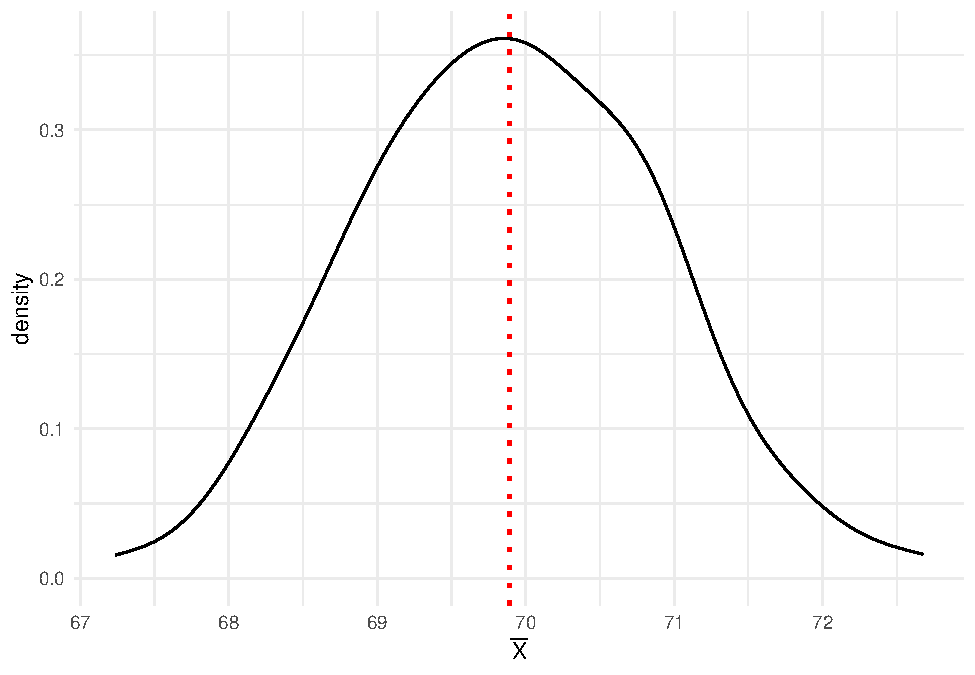
\includegraphics{Estimation-and-Confidence-intervals_files/figure-latex/unnamed-chunk-4-1.pdf}

\begin{Shaded}
\begin{Highlighting}[]
\FunctionTok{summary}\NormalTok{(vect\_mean)}
\end{Highlighting}
\end{Shaded}

\begin{verbatim}
##       Mean      
##  Min.   :67.24  
##  1st Qu.:69.21  
##  Median :69.94  
##  Mean   :69.89  
##  3rd Qu.:70.67  
##  Max.   :72.68
\end{verbatim}

We can also look at the distributions of the original sample and the
estimated means.

\begin{Shaded}
\begin{Highlighting}[]
\NormalTok{g1 }\OtherTok{\textless{}{-}} \FunctionTok{ggplot}\NormalTok{(vect\_mean)}\SpecialCharTok{+}
  \FunctionTok{geom\_histogram}\NormalTok{(}\FunctionTok{aes}\NormalTok{(}\AttributeTok{x=}\NormalTok{Mean, }\AttributeTok{y =} \FunctionTok{after\_stat}\NormalTok{(density)), }\AttributeTok{bins=}\DecValTok{15}\NormalTok{)}\SpecialCharTok{+}
  \FunctionTok{theme\_minimal}\NormalTok{()}\SpecialCharTok{+}
  \FunctionTok{xlab}\NormalTok{(}\FunctionTok{expression}\NormalTok{(}\FunctionTok{bar}\NormalTok{(x)[n])) }\SpecialCharTok{+} 
  \FunctionTok{geom\_vline}\NormalTok{(}\AttributeTok{xintercept =} \FunctionTok{mean}\NormalTok{(vect\_mean}\SpecialCharTok{$}\NormalTok{Mean), }\AttributeTok{col =} \StringTok{"red"}\NormalTok{, }\AttributeTok{linetype =} \StringTok{"dotted"}\NormalTok{, }\AttributeTok{linewidth =} \DecValTok{1}\NormalTok{) }\SpecialCharTok{+}
  \FunctionTok{geom\_density}\NormalTok{(}\FunctionTok{aes}\NormalTok{(}\AttributeTok{x =}\NormalTok{ Mean), }\AttributeTok{color =} \StringTok{"blue"}\NormalTok{, }\AttributeTok{linetype =} \StringTok{"dashed"}\NormalTok{)}
\NormalTok{g2 }\OtherTok{\textless{}{-}} \FunctionTok{ggplot}\NormalTok{()}\SpecialCharTok{+}
  \FunctionTok{geom\_histogram}\NormalTok{(}\FunctionTok{aes}\NormalTok{(}\AttributeTok{x=}\NormalTok{x, }\AttributeTok{y =} \FunctionTok{after\_stat}\NormalTok{(density)), }\AttributeTok{bins=}\DecValTok{15}\NormalTok{)}\SpecialCharTok{+}
  \FunctionTok{theme\_minimal}\NormalTok{()}\SpecialCharTok{+}
  \FunctionTok{xlab}\NormalTok{(}\FunctionTok{expression}\NormalTok{(x)) }\SpecialCharTok{+} 
  \FunctionTok{geom\_vline}\NormalTok{(}\AttributeTok{xintercept =} \FunctionTok{mean}\NormalTok{(x), }\AttributeTok{col =} \StringTok{"red"}\NormalTok{, }\AttributeTok{linetype =} \StringTok{"dotted"}\NormalTok{, }\AttributeTok{linewidth =} \DecValTok{1}\NormalTok{) }\SpecialCharTok{+}
  \FunctionTok{geom\_density}\NormalTok{(}\FunctionTok{aes}\NormalTok{(}\AttributeTok{x =}\NormalTok{ x), }\AttributeTok{color =} \StringTok{"blue"}\NormalTok{, }\AttributeTok{linetype =} \StringTok{"dashed"}\NormalTok{)}
\NormalTok{gridExtra}\SpecialCharTok{::}\FunctionTok{grid.arrange}\NormalTok{(g1,g2)}
\end{Highlighting}
\end{Shaded}

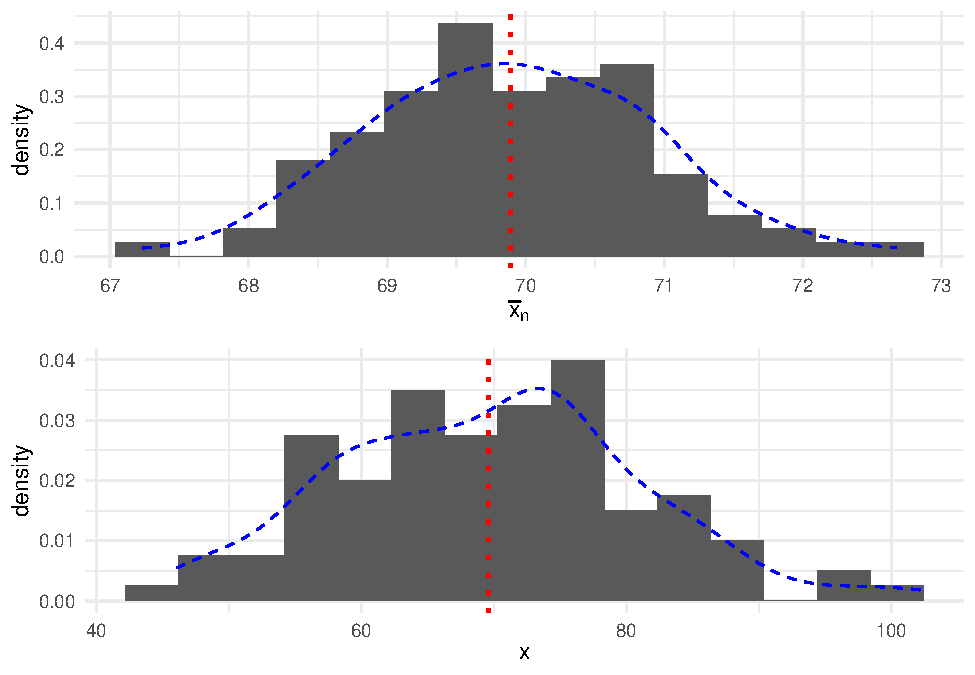
\includegraphics{Estimation-and-Confidence-intervals_files/figure-latex/unnamed-chunk-5-1.pdf}

The \emph{sampling distribution} of the estimate is the probability
distribution of the values of an estimate obtained from sampling a
population infinitely many times. Additionally, an estimator is called
unbiased if \(\mathbb{E}[\hat{\theta}] = \theta\), that is the estimator
gives ``correct'' result on average. Understanding the sampling
distribution and its properties enables us to make probabilistic
assessments of how well the statistic provides information about the
population parameter it is defined for.\\
We want estimators satisfy two crucial asymptotic properties, that hold
for increasing sample size (for the limit of \(n \to \infty\)). In
particular, consider the estimator \(\hat{\theta}_n\), where the \(n\)
indicates the dependence on the sample size, and let \(\theta\) be the
true parameter. The estimator is said to be \emph{consistent} if it
converges in probability to the true parameter value as the sample size
grows, that is
\[\hat{\theta}_n \rightarrow \theta \mbox{ as } n \to \infty\]. This
ensures that the estimate will be arbitrarily close to the true
parameter value as the sample size grows. An estimator is said to have
\emph{asymptotic normality} if
\[\sqrt{n}(\hat{\theta} - \theta) \rightarrow N(0, \sigma^2),\] that is,
for large sample sizes, the distribution of the scaled estimator
approaches a normal distribution with mean 0 and some variance
\(\sigma^2\).\\
Considering the previous figures, we can note that the sampling
distribution has a bell shape, and it has a lower spread than the
population or sample distributions, i.e.

\begin{Shaded}
\begin{Highlighting}[]
\FunctionTok{var}\NormalTok{(vect\_mean}\SpecialCharTok{$}\NormalTok{Mean)}
\end{Highlighting}
\end{Shaded}

\begin{verbatim}
## [1] 1.007442
\end{verbatim}

\begin{Shaded}
\begin{Highlighting}[]
\FunctionTok{var}\NormalTok{(x)}
\end{Highlighting}
\end{Shaded}

\begin{verbatim}
## [1] 128.1505
\end{verbatim}

The standard deviation of the distribution of an estimate is also called
\emph{standard error}, since it reflects the difference between a
parameter and the corresponding estimate. For the sample mean of a
Normal distribution, it is computed as \(\mbox{se} = s/\sqrt{n}\).

Is there any way to improve the estimate? As suggested by the asymptotic
properties, one way to improve a point estimate is to take a larger
sample, that is increasing \(n\).

\begin{Shaded}
\begin{Highlighting}[]
\NormalTok{n\_values }\OtherTok{\textless{}{-}} \FunctionTok{c}\NormalTok{(}\DecValTok{30}\NormalTok{, }\DecValTok{50}\NormalTok{, }\DecValTok{100}\NormalTok{, }\DecValTok{200}\NormalTok{)}
\NormalTok{vect\_mean }\OtherTok{\textless{}{-}} \FunctionTok{matrix}\NormalTok{(}\DecValTok{0}\NormalTok{,}\AttributeTok{nrow=}\DecValTok{400}\NormalTok{, }\AttributeTok{ncol=}\DecValTok{2}\NormalTok{)}
\NormalTok{k}\OtherTok{=}\DecValTok{0}
\ControlFlowTok{for}\NormalTok{(j }\ControlFlowTok{in}\NormalTok{ n\_values)\{}
  \ControlFlowTok{for}\NormalTok{(i }\ControlFlowTok{in} \DecValTok{1}\SpecialCharTok{:}\DecValTok{100}\NormalTok{)\{}
\NormalTok{    x }\OtherTok{\textless{}{-}} \FunctionTok{rnorm}\NormalTok{(j, }\AttributeTok{mean =} \DecValTok{70}\NormalTok{, }\AttributeTok{sd=}\DecValTok{10}\NormalTok{)}
\NormalTok{    vect\_mean[i}\SpecialCharTok{+}\NormalTok{k}\SpecialCharTok{*}\DecValTok{100}\NormalTok{,] }\OtherTok{\textless{}{-}} \FunctionTok{c}\NormalTok{(j, }\FunctionTok{mean}\NormalTok{(x))}
\NormalTok{  \}}
\NormalTok{  k }\OtherTok{=}\NormalTok{ k }\SpecialCharTok{+}\DecValTok{1}
\NormalTok{\}}
\NormalTok{vect\_mean }\OtherTok{\textless{}{-}} \FunctionTok{data.frame}\NormalTok{(vect\_mean)}
\FunctionTok{colnames}\NormalTok{(vect\_mean) }\OtherTok{\textless{}{-}} \FunctionTok{c}\NormalTok{(}\StringTok{"n"}\NormalTok{, }\StringTok{"Mean"}\NormalTok{)}
\NormalTok{vect\_mean}\SpecialCharTok{$}\NormalTok{n }\OtherTok{\textless{}{-}} \FunctionTok{as.factor}\NormalTok{(vect\_mean}\SpecialCharTok{$}\NormalTok{n)}
\FunctionTok{ggplot}\NormalTok{(vect\_mean, }\FunctionTok{aes}\NormalTok{(}\AttributeTok{x=}\NormalTok{Mean, }\AttributeTok{color=}\NormalTok{n))}\SpecialCharTok{+}
  \FunctionTok{geom\_histogram}\NormalTok{(}\AttributeTok{bins=}\DecValTok{20}\NormalTok{) }\SpecialCharTok{+}     
  \FunctionTok{facet\_grid}\NormalTok{(}\SpecialCharTok{\textasciitilde{}}\NormalTok{n)}\SpecialCharTok{+}
  \FunctionTok{geom\_vline}\NormalTok{(}\AttributeTok{xintercept =} \FunctionTok{mean}\NormalTok{(vect\_mean}\SpecialCharTok{$}\NormalTok{Mean), }\AttributeTok{col =} \StringTok{"red"}\NormalTok{, }\AttributeTok{linetype =} \StringTok{"dotted"}\NormalTok{, }\AttributeTok{size =} \DecValTok{1}\NormalTok{)}
\end{Highlighting}
\end{Shaded}

\begin{verbatim}
## Warning: Using `size` aesthetic for lines was deprecated in ggplot2 3.4.0.
## i Please use `linewidth` instead.
## This warning is displayed once every 8 hours.
## Call `lifecycle::last_lifecycle_warnings()` to see where this warning was
## generated.
\end{verbatim}

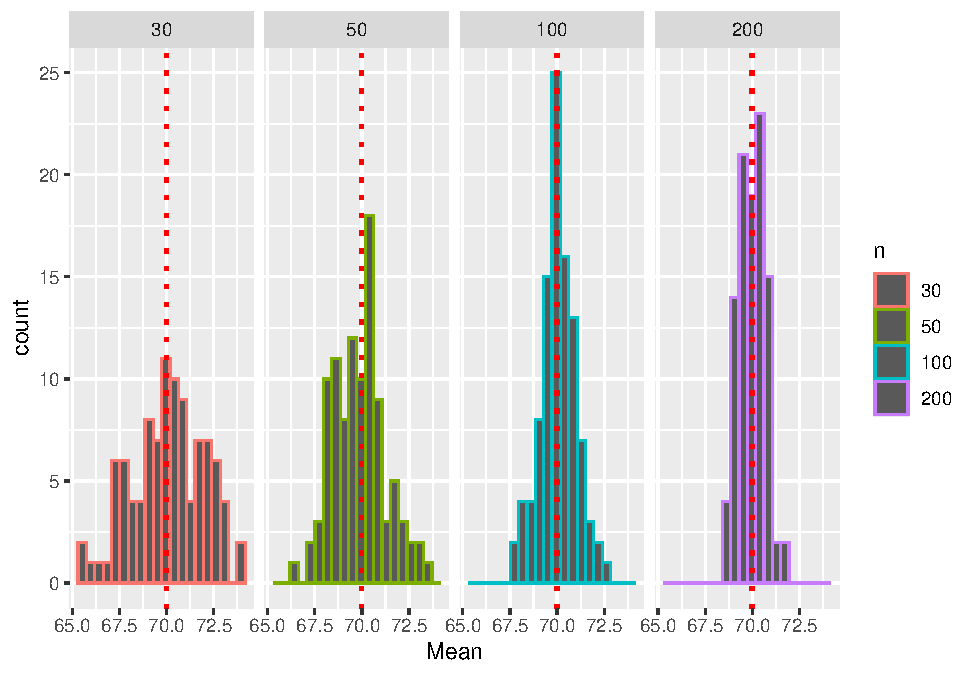
\includegraphics{Estimation-and-Confidence-intervals_files/figure-latex/unnamed-chunk-7-1.pdf}
Increasing the size of the sample decreases the variability of the
sampling distribution of the estimate. Therefore, a larger sample size
results in a more reliable point estimate of the population parameter.
The distribution of the sample mean is roughly bell-shaped (normally
distributed).

Other examples of estimators for \(\mu\) and \(\sigma^2\) are the
median, and interquartile range or median absolute deviation (MAD),
respectively.

\textbf{Remark}:

\begin{enumerate}
\def\labelenumi{(\roman{enumi})}
\item
  The sample is a subset of individuals drawn from the population.
\item
  \(X_i\) are independent and identically distributed (i.i.d.),
  following the distribution of the model described by the population:
  \(X_i \sim f(x;\theta)\).
\item
  An estimate can be also called a statistic. A \emph{statistic},
  denoted as \(T_n=T(X_1,X_2,\ldots,X_n)\), is any real-valued function
  (transformation) of the random sample \(X=(X_1,X_2,\ldots,X_n)\) that
  does not depend on any other unknown quantities. Since a statistic is
  a random variable, it has a distribution.
\item
  In statistical estimation, the sample is used to compute a single
  value, often referred to as \emph{(point) estimate}, which serves as
  the \emph{best guess} of the unknown population parameter.
\item
  The \emph{3-sigma-rule} can be also considered for the estimator
  distribution using the estimated standard error.
\end{enumerate}

\hypertarget{confidence-intervals}{%
\subsection{Confidence intervals}\label{confidence-intervals}}

Confidence intervals are a tool for quantifying the uncertainty related
to the estimated value of a parameter. Let consider again \(X\) follows
\(f(x;\theta)\), and consider a random sample \((X_1,\ldots,X_n)\) with
an estimator \(T_n=T(X_1,\ldots,X_n)\). Let \(t_n=t(x_1,\ldots,x_n)\) be
the estimate of \(\theta\). In reality, no matter how accurate the
estimator \(T_n\) is, a single number \(t_n\) (i.e., point estimate),
does not provide any indication on the probabilities that the estimate
takes on a value close or equal to the \emph{true} parameter value
\(\theta\). The \emph{\(\alpha\) confidence intervals} overcome this
inconvenience and allow us to establish a range of plausible estimates
associated with a fixed level of confidence.

In other word, it allows us to define a level of confidence \(\alpha\)
in our population parameter estimate gleaned from a sample.

Confidence interval estimation is often calculated based on the point
estimate by adding and subtracting a value known as the \emph{margin of
error}
\[ [\mbox{Point Estimate } - \mbox{ Margin of Error}; \mbox{Point Estimate } + \mbox{ Margin of Error}].\]
We want an interval that will bracket the true value of the parameter in
\((1-\alpha)\)\% of the instances of an experiment that is repeated a
large number of times.

Consider the sample mean \(\bar{X} = \frac{1}{n}\sum_{i=1}^n X_i\) and
assume the variance \(\sigma_X^2\) is known. For this estimator, we know
that the expectation and the variance are given as

\[
\mathbb{E}[\bar{X}] = \mu_X, \qquad \mathbb{E}[(\bar{X} - \mu_X)^2] = \frac{\sigma_X^2}{n}.
\] Considering the sample mean, this estimator is asymptotically normal,
that is \[
Z = \sqrt{n}\left(\frac{\bar{X} - \mu_X}{\sigma_X}\right) \rightarrow N(0,1).
\] Using this information, we can construct the \(\alpha\) confidence
intervals, with \(\alpha \in (0,1)\). Given a value \(\alpha\), we aim
to find \(u_{\alpha}\) such that
\(P(-u_{\alpha} \leq Z \leq u_{\alpha}) = 1 - \alpha\). Using the
symmetry of the normal distribution we get
\[ P\left(z_{\alpha/2} \leq \frac{\bar{X} - \mu_X}{\sigma_X} \leq z_{1-\alpha/2}\right) = 1 - \alpha\]
where \(z_b\) denotes the quantile of level \(b\) of a normal standard
distribution. Rewriting the terms with respect \(\mu\), we have that the
confidence interval for \(\mu\) at level \(1-\alpha\) is
\[IC_{1-\alpha}(\mu) = \left[ \hat{\mu} - z_{1-\alpha/2}\frac{\sigma}{\sqrt{n}}, \hat{\mu} + z_{1-\alpha/2}\frac{\sigma}{\sqrt{n}} \right],\]
where \(\hat{\mu} = \bar{x}\) is the computed sample mean estimate.

Considering the standard normal distribution, the displayed quantiles
correspond to

\begin{Shaded}
\begin{Highlighting}[]
\NormalTok{alpha }\OtherTok{\textless{}{-}} \FloatTok{0.05}
\DecValTok{1} \SpecialCharTok{{-}}\NormalTok{ alpha}
\end{Highlighting}
\end{Shaded}

\begin{verbatim}
## [1] 0.95
\end{verbatim}

\begin{Shaded}
\begin{Highlighting}[]
\FunctionTok{qnorm}\NormalTok{(alpha }\SpecialCharTok{/} \DecValTok{2}\NormalTok{) }\CommentTok{\# {-}u\_alpha}
\end{Highlighting}
\end{Shaded}

\begin{verbatim}
## [1] -1.959964
\end{verbatim}

\begin{Shaded}
\begin{Highlighting}[]
\FunctionTok{qnorm}\NormalTok{(}\DecValTok{1} \SpecialCharTok{{-}}\NormalTok{ alpha }\SpecialCharTok{/} \DecValTok{2}\NormalTok{) }\CommentTok{\# u\_alpha}
\end{Highlighting}
\end{Shaded}

\begin{verbatim}
## [1] 1.959964
\end{verbatim}

\begin{Shaded}
\begin{Highlighting}[]
\CommentTok{\# Plot confidence interval}
\FunctionTok{plot}\NormalTok{(dnorm, }\AttributeTok{from =} \SpecialCharTok{{-}}\DecValTok{5}\NormalTok{, }\AttributeTok{to =} \DecValTok{5}\NormalTok{, }\AttributeTok{main =} \StringTok{"Confidence Interval"}\NormalTok{)}
\FunctionTok{abline}\NormalTok{(}\AttributeTok{v =} \FunctionTok{qnorm}\NormalTok{(alpha }\SpecialCharTok{/} \DecValTok{2}\NormalTok{), }\AttributeTok{col =} \StringTok{"red"}\NormalTok{)}
\FunctionTok{abline}\NormalTok{(}\AttributeTok{v =} \FunctionTok{qnorm}\NormalTok{(}\DecValTok{1} \SpecialCharTok{{-}}\NormalTok{ alpha }\SpecialCharTok{/} \DecValTok{2}\NormalTok{), }\AttributeTok{col =} \StringTok{"red"}\NormalTok{)}
\end{Highlighting}
\end{Shaded}

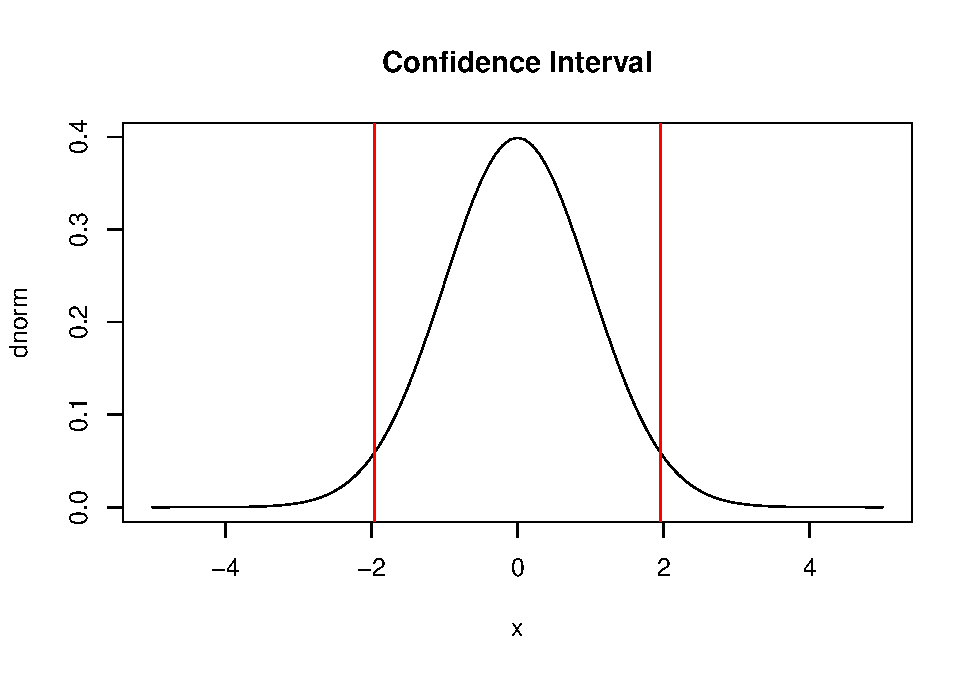
\includegraphics{Estimation-and-Confidence-intervals_files/figure-latex/unnamed-chunk-8-1.pdf}

\begin{Shaded}
\begin{Highlighting}[]
\CommentTok{\# Using ggplot}
\NormalTok{x }\OtherTok{\textless{}{-}} \FunctionTok{seq}\NormalTok{(}\SpecialCharTok{{-}}\DecValTok{4}\NormalTok{, }\DecValTok{4}\NormalTok{, }\FloatTok{0.1}\NormalTok{)}
\FunctionTok{ggplot}\NormalTok{(}\AttributeTok{mapping =} \FunctionTok{aes}\NormalTok{(}\AttributeTok{x=}\NormalTok{x, }\AttributeTok{y=}\FunctionTok{dnorm}\NormalTok{(x)))}\SpecialCharTok{+}
  \FunctionTok{geom\_line}\NormalTok{() }\SpecialCharTok{+} 
  \FunctionTok{geom\_vline}\NormalTok{(}\AttributeTok{xintercept=}\FunctionTok{qnorm}\NormalTok{(alpha}\SpecialCharTok{/}\DecValTok{2}\NormalTok{), }\AttributeTok{color=}\StringTok{"red"}\NormalTok{, }\AttributeTok{linetype=}\StringTok{"dashed"}\NormalTok{) }\SpecialCharTok{+} 
  \FunctionTok{geom\_vline}\NormalTok{(}\AttributeTok{xintercept=}\FunctionTok{qnorm}\NormalTok{(}\DecValTok{1} \SpecialCharTok{{-}}\NormalTok{ alpha}\SpecialCharTok{/}\DecValTok{2}\NormalTok{), }\AttributeTok{color=}\StringTok{"red"}\NormalTok{, }\AttributeTok{linetype=}\StringTok{"dashed"}\NormalTok{)}
\end{Highlighting}
\end{Shaded}

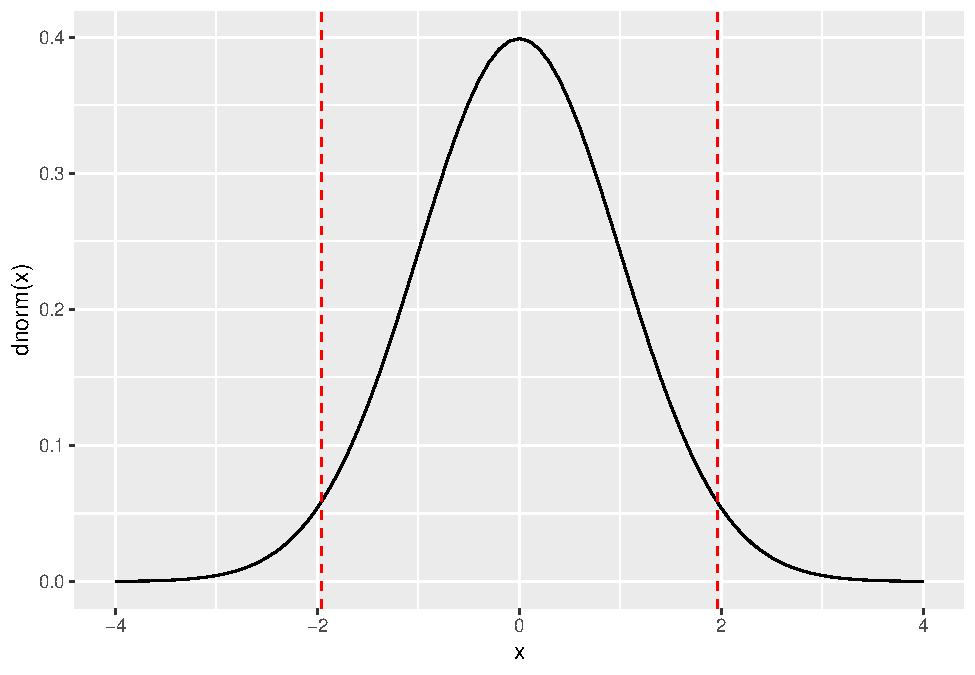
\includegraphics{Estimation-and-Confidence-intervals_files/figure-latex/unnamed-chunk-9-1.pdf}

In other words, if we estimate a lot of times the confidence intervals
from random samples, the \((1- \alpha)%
\) of the times, they include the true value of the population
parameter. For example

\begin{Shaded}
\begin{Highlighting}[]
\FunctionTok{set.seed}\NormalTok{(}\DecValTok{1234}\NormalTok{)}
\NormalTok{n }\OtherTok{\textless{}{-}} \DecValTok{100}
\NormalTok{x }\OtherTok{\textless{}{-}} \FunctionTok{rnorm}\NormalTok{(n, }\AttributeTok{mean =} \DecValTok{70}\NormalTok{, }\AttributeTok{sd =} \DecValTok{10}\NormalTok{)}
\NormalTok{mu\_x }\OtherTok{\textless{}{-}} \FunctionTok{mean}\NormalTok{(x)}
\FunctionTok{round}\NormalTok{(mu\_x,}\DecValTok{2}\NormalTok{)}
\end{Highlighting}
\end{Shaded}

\begin{verbatim}
## [1] 68.43
\end{verbatim}

\begin{Shaded}
\begin{Highlighting}[]
\NormalTok{alpha }\OtherTok{\textless{}{-}} \FloatTok{0.05}
\CommentTok{\# we assume to know that the standard deviation is equal to 10}
\NormalTok{sigma }\OtherTok{\textless{}{-}} \DecValTok{10}
\CommentTok{\# Then the confidence interval is }
\FunctionTok{round}\NormalTok{(}\FunctionTok{c}\NormalTok{(mu\_x }\SpecialCharTok{{-}} \FunctionTok{qnorm}\NormalTok{(}\DecValTok{1} \SpecialCharTok{{-}}\NormalTok{ alpha}\SpecialCharTok{/}\DecValTok{2}\NormalTok{)}\SpecialCharTok{*}\NormalTok{sigma}\SpecialCharTok{/}\FunctionTok{sqrt}\NormalTok{(n), }
\NormalTok{  mu\_x }\SpecialCharTok{+} \FunctionTok{qnorm}\NormalTok{(}\DecValTok{1} \SpecialCharTok{{-}}\NormalTok{ alpha}\SpecialCharTok{/}\DecValTok{2}\NormalTok{)}\SpecialCharTok{*}\NormalTok{sigma}\SpecialCharTok{/}\FunctionTok{sqrt}\NormalTok{(n)),}\DecValTok{2}\NormalTok{)}
\end{Highlighting}
\end{Shaded}

\begin{verbatim}
## [1] 66.47 70.39
\end{verbatim}

With this result, we can state that \emph{``We are confident at 95\%
that the true mean is inside the interval''}. But beware, people will
sometimes state this as \emph{``\ldots{} there is a 95\% chance that the
population mean falls between such and such values \ldots{}''} which is
problematic since it implies that the population mean is a random
variable when in fact it's not. The confidence interval reminds us that
the chances are in the sampling and not the population parameter.

Let's consider the data set generated in the previous generated example,
saved in \texttt{"first\_dataframe.csv"}.

\begin{Shaded}
\begin{Highlighting}[]
\NormalTok{dat }\OtherTok{\textless{}{-}} \FunctionTok{read.csv}\NormalTok{(}\StringTok{"../Exploratory Data Analysys/first\_dataframe.csv"}\NormalTok{)}
\NormalTok{dat}\SpecialCharTok{$}\NormalTok{Sex }\OtherTok{\textless{}{-}} \FunctionTok{as.factor}\NormalTok{(dat}\SpecialCharTok{$}\NormalTok{Sex)}
\NormalTok{dat}\SpecialCharTok{$}\NormalTok{Group }\OtherTok{\textless{}{-}} \FunctionTok{as.factor}\NormalTok{(dat}\SpecialCharTok{$}\NormalTok{Group)}
\end{Highlighting}
\end{Shaded}

\hypertarget{mean-with-known-variance}{%
\subsection{Mean with known variance}\label{mean-with-known-variance}}

We can see the population distribution of the \texttt{Response\_Time}
with its mean and median

\begin{Shaded}
\begin{Highlighting}[]
\FunctionTok{ggplot}\NormalTok{(dat, }\FunctionTok{aes}\NormalTok{(}\AttributeTok{x=}\NormalTok{Response\_Time))}\SpecialCharTok{+}
  \FunctionTok{geom\_density}\NormalTok{()}\SpecialCharTok{+}
  \FunctionTok{theme\_classic}\NormalTok{()}\SpecialCharTok{+}
  \FunctionTok{geom\_vline}\NormalTok{(}\AttributeTok{xintercept =} \FunctionTok{median}\NormalTok{(dat}\SpecialCharTok{$}\NormalTok{Response\_Time), }\AttributeTok{color=}\StringTok{"blue"}\NormalTok{, }\AttributeTok{linetype=}\StringTok{"dashed"}\NormalTok{, }\AttributeTok{size=}\DecValTok{1}\NormalTok{) }\SpecialCharTok{+}
  \FunctionTok{geom\_vline}\NormalTok{(}\AttributeTok{xintercept =} \FunctionTok{mean}\NormalTok{(dat}\SpecialCharTok{$}\NormalTok{Response\_Time), }\AttributeTok{color=}\StringTok{"red"}\NormalTok{,}\AttributeTok{linetype=}\StringTok{"dashed"}\NormalTok{, }\AttributeTok{size=}\DecValTok{1}\NormalTok{)}
\end{Highlighting}
\end{Shaded}

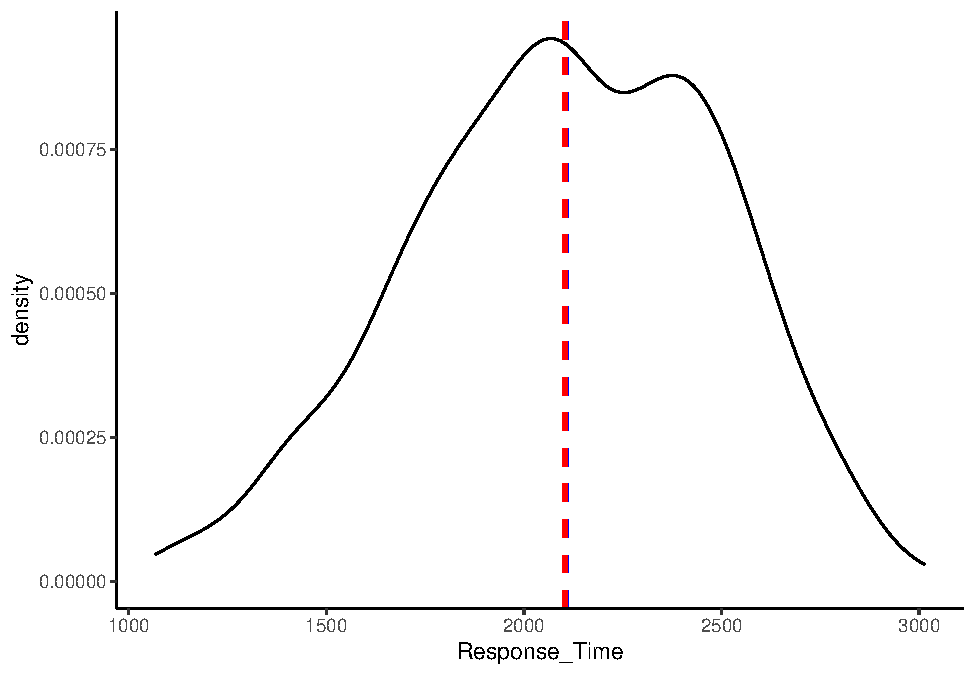
\includegraphics{Estimation-and-Confidence-intervals_files/figure-latex/unnamed-chunk-12-1.pdf}

\begin{Shaded}
\begin{Highlighting}[]
\NormalTok{x\_bar }\OtherTok{\textless{}{-}} \FunctionTok{round}\NormalTok{(}\FunctionTok{mean}\NormalTok{(dat}\SpecialCharTok{$}\NormalTok{Response\_Time),}\DecValTok{2}\NormalTok{)}
\NormalTok{s\_x }\OtherTok{\textless{}{-}} \FunctionTok{round}\NormalTok{(}\FunctionTok{sd}\NormalTok{(dat}\SpecialCharTok{$}\NormalTok{Response\_Time),}\DecValTok{2}\NormalTok{)}
\FunctionTok{print}\NormalTok{(}\FunctionTok{paste0}\NormalTok{(x\_bar, }\StringTok{" ("}\NormalTok{, s\_x, }\StringTok{")"}\NormalTok{))}
\end{Highlighting}
\end{Shaded}

\begin{verbatim}
## [1] "2104.12 (382.06)"
\end{verbatim}

\begin{Shaded}
\begin{Highlighting}[]
\FunctionTok{print}\NormalTok{(}\FunctionTok{paste0}\NormalTok{(}\FunctionTok{round}\NormalTok{(}\FunctionTok{median}\NormalTok{(dat}\SpecialCharTok{$}\NormalTok{Response\_Time),}\DecValTok{2}\NormalTok{), }\StringTok{" ("}\NormalTok{, }\FunctionTok{round}\NormalTok{(}\FunctionTok{IQR}\NormalTok{(dat}\SpecialCharTok{$}\NormalTok{Response\_Time),}\DecValTok{2}\NormalTok{), }\StringTok{")"}\NormalTok{))}
\end{Highlighting}
\end{Shaded}

\begin{verbatim}
## [1] "2107.06 (566.5)"
\end{verbatim}

Let's compute the 95\% confidence interval, considering the variance
known.

\begin{Shaded}
\begin{Highlighting}[]
\NormalTok{mean\_R }\OtherTok{\textless{}{-}} \FunctionTok{mean}\NormalTok{(dat}\SpecialCharTok{$}\NormalTok{Response\_Time)}
\CommentTok{\# We round the standard deviation just for supposing that the variance is known.}
\NormalTok{sd\_R }\OtherTok{\textless{}{-}} \FunctionTok{round}\NormalTok{(}\FunctionTok{sd}\NormalTok{(dat}\SpecialCharTok{$}\NormalTok{Response\_Time))}
\NormalTok{n }\OtherTok{\textless{}{-}} \FunctionTok{nrow}\NormalTok{(dat)}
\NormalTok{alpha }\OtherTok{\textless{}{-}} \FloatTok{0.05}
\NormalTok{lb }\OtherTok{\textless{}{-}} \FunctionTok{round}\NormalTok{(mean\_R }\SpecialCharTok{{-}} \FunctionTok{qnorm}\NormalTok{(}\DecValTok{1}\SpecialCharTok{{-}}\NormalTok{alpha}\SpecialCharTok{/}\DecValTok{2}\NormalTok{)}\SpecialCharTok{*}\NormalTok{sd\_R}\SpecialCharTok{/}\FunctionTok{sqrt}\NormalTok{(n), }\AttributeTok{digits =} \DecValTok{3}\NormalTok{)}
\NormalTok{rb }\OtherTok{\textless{}{-}} \FunctionTok{round}\NormalTok{(mean\_R }\SpecialCharTok{+} \FunctionTok{qnorm}\NormalTok{(}\DecValTok{1}\SpecialCharTok{{-}}\NormalTok{alpha}\SpecialCharTok{/}\DecValTok{2}\NormalTok{)}\SpecialCharTok{*}\NormalTok{sd\_R}\SpecialCharTok{/}\FunctionTok{sqrt}\NormalTok{(n), }\AttributeTok{digits =} \DecValTok{3}\NormalTok{)}
\FunctionTok{print}\NormalTok{(}\FunctionTok{paste0}\NormalTok{(}\StringTok{"The confidence interval for the estimate "}\NormalTok{, mean\_R, }\StringTok{" is ["}\NormalTok{, lb, }\StringTok{";"}\NormalTok{, rb, }\StringTok{"]"}\NormalTok{))}
\end{Highlighting}
\end{Shaded}

\begin{verbatim}
## [1] "The confidence interval for the estimate 2104.1201142988 is [2070.637;2137.603]"
\end{verbatim}

With this result we can state: \emph{We are confident at 95\% that the
true mean is inside this interval}.

\hypertarget{example}{%
\paragraph{Example}\label{example}}

Let's consider an example where a metallurgical industry produces plates
with a thickness of \(14 \text{mm}\) and a tolerance of
\(0.5 \text{mm}\). Every shift (every 6 hours), 10 plates are sampled
and their thickness is measured.

\begin{Shaded}
\begin{Highlighting}[]
\NormalTok{thickness }\OtherTok{\textless{}{-}} \FunctionTok{c}\NormalTok{(}\FloatTok{13.88}\NormalTok{, }\FloatTok{14.03}\NormalTok{, }\FloatTok{14.11}\NormalTok{, }\FloatTok{13.77}\NormalTok{, }\FloatTok{14.04}\NormalTok{, }\FloatTok{14.05}\NormalTok{, }\FloatTok{13.94}\NormalTok{, }\FloatTok{13.95}\NormalTok{, }\FloatTok{13.94}\NormalTok{, }\FloatTok{13.91}\NormalTok{)}
\NormalTok{alpha }\OtherTok{\textless{}{-}} \FloatTok{0.05}
\NormalTok{Var }\OtherTok{\textless{}{-}} \FloatTok{0.01}
\NormalTok{x\_bar }\OtherTok{\textless{}{-}} \FunctionTok{mean}\NormalTok{(thickness)}
\NormalTok{n }\OtherTok{\textless{}{-}} \FunctionTok{length}\NormalTok{(thickness)}
\NormalTok{u\_alpha }\OtherTok{\textless{}{-}} \FunctionTok{qnorm}\NormalTok{(}\DecValTok{1} \SpecialCharTok{{-}}\NormalTok{ alpha }\SpecialCharTok{/} \DecValTok{2}\NormalTok{)}
\NormalTok{conf\_interval }\OtherTok{\textless{}{-}} \FunctionTok{c}\NormalTok{(x\_bar }\SpecialCharTok{{-}}\NormalTok{ u\_alpha }\SpecialCharTok{*} \FunctionTok{sqrt}\NormalTok{(Var }\SpecialCharTok{/}\NormalTok{ n), x\_bar }\SpecialCharTok{+}\NormalTok{ u\_alpha }\SpecialCharTok{*} \FunctionTok{sqrt}\NormalTok{(Var }\SpecialCharTok{/}\NormalTok{ n))}
\NormalTok{conf\_interval}
\end{Highlighting}
\end{Shaded}

\begin{verbatim}
## [1] 13.90002 14.02398
\end{verbatim}

By changing the value of \(\alpha\), intervals with different confidence
levels can be obtained.

\begin{Shaded}
\begin{Highlighting}[]
\NormalTok{alpha }\OtherTok{\textless{}{-}} \FloatTok{0.01}
\NormalTok{u\_alpha }\OtherTok{\textless{}{-}} \FunctionTok{qnorm}\NormalTok{(}\DecValTok{1} \SpecialCharTok{{-}}\NormalTok{ alpha }\SpecialCharTok{/} \DecValTok{2}\NormalTok{)}
\NormalTok{conf\_interval }\OtherTok{\textless{}{-}} \FunctionTok{c}\NormalTok{(x\_bar }\SpecialCharTok{{-}}\NormalTok{ u\_alpha }\SpecialCharTok{*} \FunctionTok{sqrt}\NormalTok{(Var }\SpecialCharTok{/}\NormalTok{ n), x\_bar }\SpecialCharTok{+}\NormalTok{ u\_alpha }\SpecialCharTok{*} \FunctionTok{sqrt}\NormalTok{(Var }\SpecialCharTok{/}\NormalTok{ n))}
\NormalTok{conf\_interval}
\end{Highlighting}
\end{Shaded}

\begin{verbatim}
## [1] 13.88055 14.04345
\end{verbatim}

\textbf{Remark:} If the variance is unknown, but the sample size is
large, the required variance for constructing the confidence interval
can be approximated using the sample variance.

\hypertarget{mean-with-unknown-variance}{%
\subsection{Mean with Unknown
Variance}\label{mean-with-unknown-variance}}

Now, let us consider the case where the variance \(\sigma^2\) is
unknown. In this case, we estimate \(\sigma^2\) by using a proper
estimator, that could be
\[s^2 = \frac{1}{n-1}\sum_{i=1}^n(X_i - \bar{X})^2\] where \(s\) is the
sample standard deviation. The variance of the mean
\(\sigma^2_X = \sigma^2/n\) then it can be estimated as
\(s^2_X = s^2/n\). This introduces an additional level of uncertainty
and the complication that, for small samples the sample estimate of
standard deviation tend to be biased compared to the true population
standard deviation.\\
In the case of small sample sizes and unknown standard deviation,
instead of using the normal distribution, it is appropriate to use the
quantiles of the \emph{Student's t-distribution}, characterized by a
single parameter of degrees of freedom \(df = n-1\). For increasing
\(df\), the t-distributions becomes more and more similar to the
standard normal distribution.

The confidence interval is computed as in the previous case using the
sample standard deviation
\[IC_{1-\alpha}(\mu) = \left[ \hat{\mu} - t_{1-\alpha/2}\frac{\hat\sigma}{\sqrt{n}}, \hat{\mu} + t_{1-\alpha/2}\frac{\hat\sigma}{\sqrt{n}} \right].\]

\hypertarget{example.}{%
\paragraph{Example.}\label{example.}}

A wholesale supplier of bathroom fixtures wants to maintain internal
control over sales. To do so, invoices must be accompanied by a transfer
receipt to remove goods from the warehouse. At the end of each month, a
sample of invoices is taken to evaluate the average amount reported.
Over the last 5 years, the average invoice amount has been \$120. Given
that transport costs are influenced by delivery distance, it is
important to monitor the average amount. Consider the following sample:

\begin{Shaded}
\begin{Highlighting}[]
\NormalTok{fatture }\OtherTok{\textless{}{-}} \FunctionTok{c}\NormalTok{(}\FloatTok{108.98}\NormalTok{, }\FloatTok{152.22}\NormalTok{, }\FloatTok{111.45}\NormalTok{, }\FloatTok{110.59}\NormalTok{, }\FloatTok{127.46}\NormalTok{, }\FloatTok{107.26}\NormalTok{, }\FloatTok{93.32}\NormalTok{, }
             \FloatTok{91.97}\NormalTok{, }\FloatTok{111.56}\NormalTok{, }\FloatTok{75.71}\NormalTok{, }\FloatTok{128.58}\NormalTok{, }\FloatTok{135.11}\NormalTok{)}
\NormalTok{fatture}
\end{Highlighting}
\end{Shaded}

\begin{verbatim}
##  [1] 108.98 152.22 111.45 110.59 127.46 107.26  93.32  91.97 111.56  75.71
## [11] 128.58 135.11
\end{verbatim}

We assume the distribution of the amounts, described by the random
variable \(X\), can be approximated by a normal distribution,
\(X \sim N(\mu_X, \sigma^2_X)\).

Note: In practice, the assumption that data follows a normal
distribution must be verified. There are graphical and analytical
methods to assess the ``normality'' of the data distribution.

We compute the sample mean \(\bar{X}\) and the sample variance \(S^2\):

\begin{Shaded}
\begin{Highlighting}[]
\NormalTok{mx }\OtherTok{\textless{}{-}} \FunctionTok{mean}\NormalTok{(fatture)}
\NormalTok{s2 }\OtherTok{\textless{}{-}} \FunctionTok{var}\NormalTok{(fatture)}
\NormalTok{mx}
\end{Highlighting}
\end{Shaded}

\begin{verbatim}
## [1] 112.8508
\end{verbatim}

\begin{Shaded}
\begin{Highlighting}[]
\NormalTok{s2}
\end{Highlighting}
\end{Shaded}

\begin{verbatim}
## [1] 432.5565
\end{verbatim}

In this case, we do not know the true value of \(\sigma^2_X\). Given the
sample size \(n\) and sample variance \(S^2\), we know that:
\[t = \sqrt{n}\frac{X - \bar{X}}{\sqrt{S^2}} \sim t_{n-1}\] follows a
\(t\)-distribution with \(n-1\) degrees of freedom. To construct the
confidence interval for the sample mean, we calculate the quantile of a
\(t\)-distribution with \(n-1\) degrees of freedom. In our example:

\begin{Shaded}
\begin{Highlighting}[]
\NormalTok{n }\OtherTok{\textless{}{-}} \FunctionTok{length}\NormalTok{(fatture)}
\NormalTok{alpha }\OtherTok{\textless{}{-}} \FloatTok{0.01}
\NormalTok{z }\OtherTok{\textless{}{-}} \FunctionTok{qt}\NormalTok{(}\DecValTok{1} \SpecialCharTok{{-}}\NormalTok{ alpha }\SpecialCharTok{/} \DecValTok{2}\NormalTok{, n }\SpecialCharTok{{-}} \DecValTok{1}\NormalTok{)}
\NormalTok{interval }\OtherTok{\textless{}{-}} \FunctionTok{c}\NormalTok{(mx }\SpecialCharTok{{-}}\NormalTok{ z }\SpecialCharTok{*} \FunctionTok{sqrt}\NormalTok{(s2 }\SpecialCharTok{/}\NormalTok{ n), mx }\SpecialCharTok{+}\NormalTok{ z }\SpecialCharTok{*} \FunctionTok{sqrt}\NormalTok{(s2 }\SpecialCharTok{/}\NormalTok{ n))}
\NormalTok{interval}
\end{Highlighting}
\end{Shaded}

\begin{verbatim}
## [1]  94.2040 131.4977
\end{verbatim}

In R, there are functions to calculate confidence intervals directly,
while performing hypothesis tests. For example, the \texttt{t.test}
function allows you to input the sample and the confidence level with
conf.level. For instance:

\begin{Shaded}
\begin{Highlighting}[]
\FunctionTok{t.test}\NormalTok{(fatture, }\AttributeTok{conf.level =} \FloatTok{0.99}\NormalTok{)}
\end{Highlighting}
\end{Shaded}

\begin{verbatim}
## 
##  One Sample t-test
## 
## data:  fatture
## t = 18.796, df = 11, p-value = 1.039e-09
## alternative hypothesis: true mean is not equal to 0
## 99 percent confidence interval:
##   94.2040 131.4977
## sample estimates:
## mean of x 
##  112.8508
\end{verbatim}

The displayed confidence interval matches with the previously computed
interval.

\hypertarget{variance-parameter}{%
\subsection{Variance parameter}\label{variance-parameter}}

For the sample variance, we know that:

\[
\frac{(n-1)s^2}{\sigma^2_X} \sim \chi^2_{n-1}
\]

where \(\chi^2_{n-1}\) denotes the chi-squared distribution with \(n-1\)
degrees of freedom.

\begin{Shaded}
\begin{Highlighting}[]
\CommentTok{\# The chi{-}squared distribution}
\NormalTok{x}\OtherTok{=}\FunctionTok{seq}\NormalTok{(}\DecValTok{0}\NormalTok{,}\DecValTok{30}\NormalTok{,}\FloatTok{0.1}\NormalTok{)}
\FunctionTok{ggplot}\NormalTok{(}\AttributeTok{mapping =} \FunctionTok{aes}\NormalTok{(}\AttributeTok{x=}\NormalTok{x)) }\SpecialCharTok{+}
  \FunctionTok{geom\_line}\NormalTok{(}\AttributeTok{mapping =} \FunctionTok{aes}\NormalTok{(}\AttributeTok{y=}\FunctionTok{dchisq}\NormalTok{(x, }\AttributeTok{df =} \DecValTok{3}\NormalTok{)))}\SpecialCharTok{+}
  \FunctionTok{geom\_line}\NormalTok{(}\AttributeTok{mapping =} \FunctionTok{aes}\NormalTok{(}\AttributeTok{y=}\FunctionTok{dchisq}\NormalTok{(x, }\AttributeTok{df =} \DecValTok{5}\NormalTok{)), }\AttributeTok{color =} \StringTok{"blue"}\NormalTok{)}\SpecialCharTok{+}
  \FunctionTok{geom\_line}\NormalTok{(}\AttributeTok{mapping =} \FunctionTok{aes}\NormalTok{(}\AttributeTok{y=}\FunctionTok{dchisq}\NormalTok{(x, }\AttributeTok{df =} \DecValTok{10}\NormalTok{)), }\AttributeTok{color =} \StringTok{"purple"}\NormalTok{)}\SpecialCharTok{+}
  \FunctionTok{geom\_line}\NormalTok{(}\AttributeTok{mapping =} \FunctionTok{aes}\NormalTok{(}\AttributeTok{y=}\FunctionTok{dchisq}\NormalTok{(x, }\AttributeTok{df =} \DecValTok{20}\NormalTok{)), }\AttributeTok{color =} \StringTok{"red"}\NormalTok{)}
\end{Highlighting}
\end{Shaded}

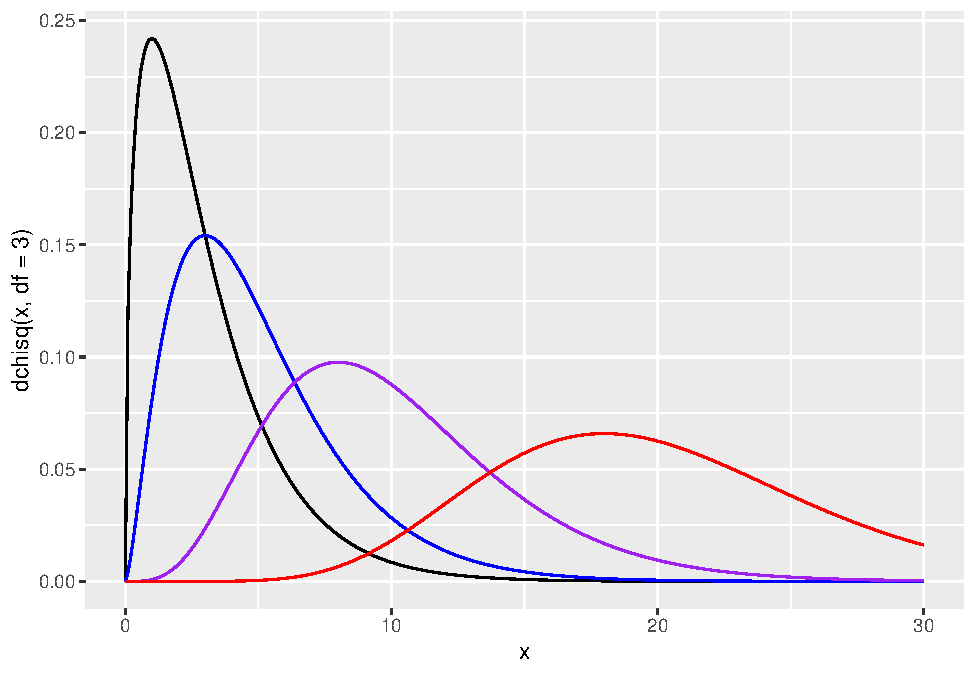
\includegraphics{Estimation-and-Confidence-intervals_files/figure-latex/unnamed-chunk-20-1.pdf}

To construct a confidence interval for the sample variance, we use the
quantiles of a chi-squared distribution
\[IC_{1-\alpha}(\sigma^2) = \left[ s^2 \frac{df}{\chi^2_{\alpha/2, df}}, s^2 \frac{df}{\chi^2_{1 - \alpha/2, df}} \right].\]
For example:

\begin{Shaded}
\begin{Highlighting}[]
\NormalTok{x }\OtherTok{\textless{}{-}} \FunctionTok{c}\NormalTok{(}\FloatTok{0.39}\NormalTok{, }\FloatTok{0.68}\NormalTok{, }\FloatTok{0.82}\NormalTok{, }\FloatTok{1.35}\NormalTok{, }\FloatTok{1.38}\NormalTok{, }\FloatTok{1.62}\NormalTok{, }\FloatTok{1.70}\NormalTok{, }\FloatTok{1.71}\NormalTok{, }\FloatTok{1.85}\NormalTok{, }\FloatTok{2.14}\NormalTok{, }\FloatTok{2.89}\NormalTok{, }\FloatTok{3.69}\NormalTok{)}
\NormalTok{s2 }\OtherTok{\textless{}{-}} \FunctionTok{var}\NormalTok{(x)}
\NormalTok{s2}
\end{Highlighting}
\end{Shaded}

\begin{verbatim}
## [1] 0.8501727
\end{verbatim}

Now, we compute the confidence interval for the variance:

\begin{Shaded}
\begin{Highlighting}[]
\NormalTok{conf\_level }\OtherTok{\textless{}{-}} \FloatTok{0.95}
\NormalTok{alpha }\OtherTok{\textless{}{-}} \DecValTok{1} \SpecialCharTok{{-}}\NormalTok{ conf\_level}
\NormalTok{n }\OtherTok{\textless{}{-}} \FunctionTok{length}\NormalTok{(x)}
\NormalTok{interval }\OtherTok{\textless{}{-}} \FunctionTok{c}\NormalTok{((n}\DecValTok{{-}1}\NormalTok{) }\SpecialCharTok{*}\NormalTok{ s2 }\SpecialCharTok{/} \FunctionTok{qchisq}\NormalTok{(}\DecValTok{1} \SpecialCharTok{{-}}\NormalTok{ alpha }\SpecialCharTok{/} \DecValTok{2}\NormalTok{, n }\SpecialCharTok{{-}} \DecValTok{1}\NormalTok{), }
\NormalTok{              (n}\DecValTok{{-}1}\NormalTok{) }\SpecialCharTok{*}\NormalTok{ s2 }\SpecialCharTok{/} \FunctionTok{qchisq}\NormalTok{(alpha }\SpecialCharTok{/} \DecValTok{2}\NormalTok{, n }\SpecialCharTok{{-}} \DecValTok{1}\NormalTok{))}
\NormalTok{interval}
\end{Highlighting}
\end{Shaded}

\begin{verbatim}
## [1] 0.4266368 2.4508692
\end{verbatim}

\hypertarget{proportions}{%
\subsection{Proportions}\label{proportions}}

So far, we have considered confidence intervals and hypothesis tests for
the mean and variance of Gaussian random variables. Now, let us consider
the case of a Bernoulli and binomial distributions.

The proportion is the most important descriptive statistic for a
categorical variable.\\
Given the random variable \(X \sim Ber(\pi)\) and the sample
\(X_1, \ldots, X_n\) from \(X\), the sample mean or \emph{sample
proportion} represents the proportion of successes in the random sample.
It is computed as
\[\hat{p} = \frac{\mbox{number of observations in the category}}{n}.\]
Note that \(\hat p\) represents the proportion of success \emph{on
average}. The standard error of \(\hat p\) is given as
\[\sigma_{\hat p} = \sqrt{\frac{\pi (1-\pi)}{n}}.\] The sampling
distribution of \(\hat{p}\) can be approximated by a Normal distribution
\[\hat{p} \approx N(p, p(1-p)/n)\] with \(n\) sufficiently large. The
confidence interval for the proportion of a population is
\[IC_{1-\alpha}(p) = \left[ \hat{p} - z_{1-\alpha/2}\sqrt{\frac{\hat{p}(1 - \hat{p})}{n}}, \hat{p} + z_{1-\alpha/2}\sqrt{\frac{\hat{p}(1 - \hat{p})}{n}} \right].\]

For example

\begin{Shaded}
\begin{Highlighting}[]
\NormalTok{group }\OtherTok{\textless{}{-}} \FunctionTok{c}\NormalTok{(}\StringTok{"Case"}\NormalTok{, }\StringTok{"Control"}\NormalTok{, }\StringTok{"Control"}\NormalTok{, }\StringTok{"Case"}\NormalTok{, }\StringTok{"Control"}\NormalTok{, }\StringTok{"Case"}\NormalTok{, }\StringTok{"Control"}\NormalTok{, }\StringTok{"Case"}\NormalTok{, }\StringTok{"Control"}\NormalTok{, }\StringTok{"Control"}\NormalTok{, }\StringTok{"Control"}\NormalTok{, }\StringTok{"Case"}\NormalTok{, }\StringTok{"Case"}\NormalTok{,}\StringTok{"Case"}\NormalTok{, }\StringTok{"Case"}\NormalTok{, }\StringTok{"Control"}\NormalTok{, }\StringTok{"Case"}\NormalTok{, }\StringTok{"Control"}\NormalTok{, }\StringTok{"Control"}\NormalTok{, }\StringTok{"Case"}\NormalTok{, }\StringTok{"Control"}\NormalTok{, }\StringTok{"Control"}\NormalTok{)}
\NormalTok{n }\OtherTok{\textless{}{-}} \FunctionTok{length}\NormalTok{(group)}
\NormalTok{p\_control }\OtherTok{\textless{}{-}} \FunctionTok{length}\NormalTok{(group[}\FunctionTok{which}\NormalTok{(group }\SpecialCharTok{==} \StringTok{"Case"}\NormalTok{)])}\SpecialCharTok{/}\NormalTok{n}
\NormalTok{p\_control}
\end{Highlighting}
\end{Shaded}

\begin{verbatim}
## [1] 0.4545455
\end{verbatim}

We computed the proportion of subject in the Control group and now we
compute the related confidence interval

\begin{Shaded}
\begin{Highlighting}[]
\NormalTok{alpha }\OtherTok{\textless{}{-}} \FloatTok{0.05}
\NormalTok{se }\OtherTok{\textless{}{-}} \FunctionTok{sqrt}\NormalTok{(p\_control }\SpecialCharTok{*}\NormalTok{ (}\DecValTok{1} \SpecialCharTok{{-}}\NormalTok{ p\_control) }\SpecialCharTok{/}\NormalTok{ (n}\DecValTok{{-}1}\NormalTok{))}
\NormalTok{u\_alpha }\OtherTok{\textless{}{-}} \FunctionTok{qnorm}\NormalTok{(}\DecValTok{1} \SpecialCharTok{{-}}\NormalTok{ alpha}\SpecialCharTok{/}\DecValTok{2}\NormalTok{)}
\NormalTok{interval }\OtherTok{\textless{}{-}} \FunctionTok{c}\NormalTok{(p\_control }\SpecialCharTok{{-}}\NormalTok{ u\_alpha}\SpecialCharTok{*}\NormalTok{se,}
\NormalTok{              p\_control }\SpecialCharTok{+}\NormalTok{ u\_alpha}\SpecialCharTok{*}\NormalTok{se)}
\NormalTok{interval}
\end{Highlighting}
\end{Shaded}

\begin{verbatim}
## [1] 0.2415814 0.6675095
\end{verbatim}

\begin{Shaded}
\begin{Highlighting}[]
\CommentTok{\# This corresponds to the Wald method}
\end{Highlighting}
\end{Shaded}

We can do this using the \texttt{prop.test} function. This function
requires a table with the counts.

\begin{Shaded}
\begin{Highlighting}[]
\FunctionTok{prop.test}\NormalTok{(}\FunctionTok{table}\NormalTok{(group), }\AttributeTok{conf.level =} \FloatTok{0.95}\NormalTok{)}
\end{Highlighting}
\end{Shaded}

\begin{verbatim}
## 
##  1-sample proportions test with continuity correction
## 
## data:  table(group), null probability 0.5
## X-squared = 0.045455, df = 1, p-value = 0.8312
## alternative hypothesis: true p is not equal to 0.5
## 95 percent confidence interval:
##  0.2507068 0.6732606
## sample estimates:
##         p 
## 0.4545455
\end{verbatim}

\hypertarget{example-political-candidate}{%
\paragraph{Example: Political
Candidate}\label{example-political-candidate}}

A politician wants to run for office in a district with 100,000 voters.
Before announcing the candidacy, they want to assess their likelihood of
success. To do this, a survey company is hired to contact 2,500 voters.
Out of these, 1,328 declare themselves in favor of the candidate, which
corresponds to a percentage of:

\[
\frac{1328}{2500} \cdot 100\% = 53\%.
\]

We want to infer the unknown percentage \(p\) of voters favoring the
candidate. The assumptions are:

\begin{itemize}
\tightlist
\item
  All respondents have the same probability of being included in the
  sample.
\item
  Responses are independent (no influence among respondents).
\end{itemize}

Under these conditions, the number of supporters \(y\) among the \(n\)
surveyed voters can be modeled as a random variable
\(Y \sim Bin(n, p)\). An estimate is given by:

\begin{Shaded}
\begin{Highlighting}[]
\NormalTok{n }\OtherTok{\textless{}{-}} \DecValTok{2500}
\NormalTok{y }\OtherTok{\textless{}{-}} \DecValTok{1328}
\NormalTok{p\_hat }\OtherTok{\textless{}{-}}\NormalTok{ y }\SpecialCharTok{/}\NormalTok{ n}
\NormalTok{p\_hat}
\end{Highlighting}
\end{Shaded}

\begin{verbatim}
## [1] 0.5312
\end{verbatim}

In general, the confidence interval is constructed using the normal
approximation \[\frac{\hat{p}-p}{\sqrt{p(1-p)}/\sqrt{n}} \sim N(0,1),\]
hence:

\begin{Shaded}
\begin{Highlighting}[]
\NormalTok{alpha }\OtherTok{\textless{}{-}} \FloatTok{0.1}
\NormalTok{Var }\OtherTok{\textless{}{-}}\NormalTok{ p\_hat }\SpecialCharTok{*}\NormalTok{ (}\DecValTok{1} \SpecialCharTok{{-}}\NormalTok{ p\_hat) }\SpecialCharTok{/}\NormalTok{ n}
\NormalTok{interval }\OtherTok{\textless{}{-}} \FunctionTok{c}\NormalTok{(p\_hat }\SpecialCharTok{{-}} \FunctionTok{qnorm}\NormalTok{(}\DecValTok{1} \SpecialCharTok{{-}}\NormalTok{ alpha }\SpecialCharTok{/} \DecValTok{2}\NormalTok{) }\SpecialCharTok{*} \FunctionTok{sqrt}\NormalTok{(Var), }
\NormalTok{              p\_hat }\SpecialCharTok{+} \FunctionTok{qnorm}\NormalTok{(}\DecValTok{1} \SpecialCharTok{{-}}\NormalTok{ alpha }\SpecialCharTok{/} \DecValTok{2}\NormalTok{) }\SpecialCharTok{*} \FunctionTok{sqrt}\NormalTok{(Var))}
\NormalTok{interval}
\end{Highlighting}
\end{Shaded}

\begin{verbatim}
## [1] 0.5147835 0.5476165
\end{verbatim}

Given this result, the politician may conclude that there is a
reasonable expectation of winning.

\hypertarget{comparison-of-means-of-two-normal-populations}{%
\subsection{Comparison of Means of Two Normal
Populations}\label{comparison-of-means-of-two-normal-populations}}

Until now, we have considered the case of a single population. Once the
measures of central tendency and variability have been calculated, we
have tested the reliability of these estimates using confidence
intervals. Now, we will consider cases where there are two or more
populations, and the goal is to perform inference by comparing them.

When the difference in population means is analyzed, we must think about
the type of sampling design we have:

\begin{enumerate}
\def\labelenumi{(\roman{enumi})}
\tightlist
\item
  Design with independent random samples,
\item
  Paired sampling design.
\end{enumerate}

These two sampling designs result in differences in the methods used to
compare the two populations.\\
Consider two independent random variables \(X_1\) and \(X_2\), and
corresponding samples of size \(n_1\) and \(n_2\), respectively. We
assume that \(X_1\sim N(\mu_1,\sigma_1)\) and
\(X_2\sim N(\mu_2,\sigma_2)\). We can consider the difference
\(\mu_1 - \mu_2\) and the results seen for testing the mean estimate of
a normally distributed random variable apply.

As in the case of a single mean \(\mu\), if we use an estimate of
\(\sigma^2_1\) and \(\sigma^2_2\) instead of the true population value
inside the confidence interval formulation, we must consider the
quantile of the student \(t\)-distribution instead of the standard
normal one. In this case the degrees of freedom \(df = n_1 + n_2 -2\)
for the second case, while the in the first case has a more complicated
formula that we will not consider here.

\hypertarget{example-wage-comparison-between-unionized-and-non-unionized-women}{%
\paragraph{Example: Wage Comparison Between Unionized and Non-Unionized
Women}\label{example-wage-comparison-between-unionized-and-non-unionized-women}}

The Wall Street Journal on July 26, 1994, stated:

\emph{``Women who are union members earn \$2.50 per hour more than women
who are not union members.''}

Based on this statement, it seems advantageous for women in the U.S. to
be part of a union. Suppose we have samples of wages for women who are
union members and those who are not:

\begin{Shaded}
\begin{Highlighting}[]
\NormalTok{iscritte }\OtherTok{\textless{}{-}} \FunctionTok{c}\NormalTok{(}\FloatTok{22.40}\NormalTok{, }\FloatTok{18.90}\NormalTok{, }\FloatTok{16.70}\NormalTok{, }\FloatTok{14.05}\NormalTok{, }\FloatTok{16.20}\NormalTok{, }\FloatTok{20.00}\NormalTok{, }\FloatTok{16.10}\NormalTok{, }\FloatTok{16.30}\NormalTok{, }\FloatTok{19.10}\NormalTok{, }\FloatTok{16.50}\NormalTok{, }\FloatTok{18.50}\NormalTok{, }\FloatTok{19.80}\NormalTok{, }\FloatTok{17.00}\NormalTok{, }\FloatTok{14.30}\NormalTok{, }\FloatTok{17.20}\NormalTok{)}
\NormalTok{non\_iscritte }\OtherTok{\textless{}{-}} \FunctionTok{c}\NormalTok{(}\FloatTok{17.60}\NormalTok{, }\FloatTok{14.40}\NormalTok{, }\FloatTok{16.60}\NormalTok{, }\FloatTok{15.00}\NormalTok{, }\FloatTok{17.65}\NormalTok{, }\FloatTok{15.00}\NormalTok{, }\FloatTok{17.55}\NormalTok{, }\FloatTok{13.30}\NormalTok{, }\FloatTok{11.20}\NormalTok{, }\FloatTok{15.90}\NormalTok{, }\FloatTok{19.20}\NormalTok{, }\FloatTok{11.85}\NormalTok{, }\FloatTok{16.65}\NormalTok{, }\FloatTok{15.20}\NormalTok{, }\FloatTok{15.30}\NormalTok{, }\FloatTok{17.00}\NormalTok{, }\FloatTok{15.10}\NormalTok{, }\FloatTok{14.30}\NormalTok{, }\FloatTok{13.90}\NormalTok{, }\FloatTok{14.50}\NormalTok{)}
\FunctionTok{length}\NormalTok{(iscritte)}
\end{Highlighting}
\end{Shaded}

\begin{verbatim}
## [1] 15
\end{verbatim}

\begin{Shaded}
\begin{Highlighting}[]
\FunctionTok{length}\NormalTok{(non\_iscritte)}
\end{Highlighting}
\end{Shaded}

\begin{verbatim}
## [1] 20
\end{verbatim}

We note that the two samples have different sizes. Descriptive
statistics and visualizations can be helpful for initial comparisons:

\begin{Shaded}
\begin{Highlighting}[]
\FunctionTok{boxplot}\NormalTok{(iscritte, non\_iscritte, }\AttributeTok{names =} \FunctionTok{c}\NormalTok{(}\StringTok{"Unionized"}\NormalTok{, }\StringTok{"Non{-}Unionized"}\NormalTok{))}
\end{Highlighting}
\end{Shaded}

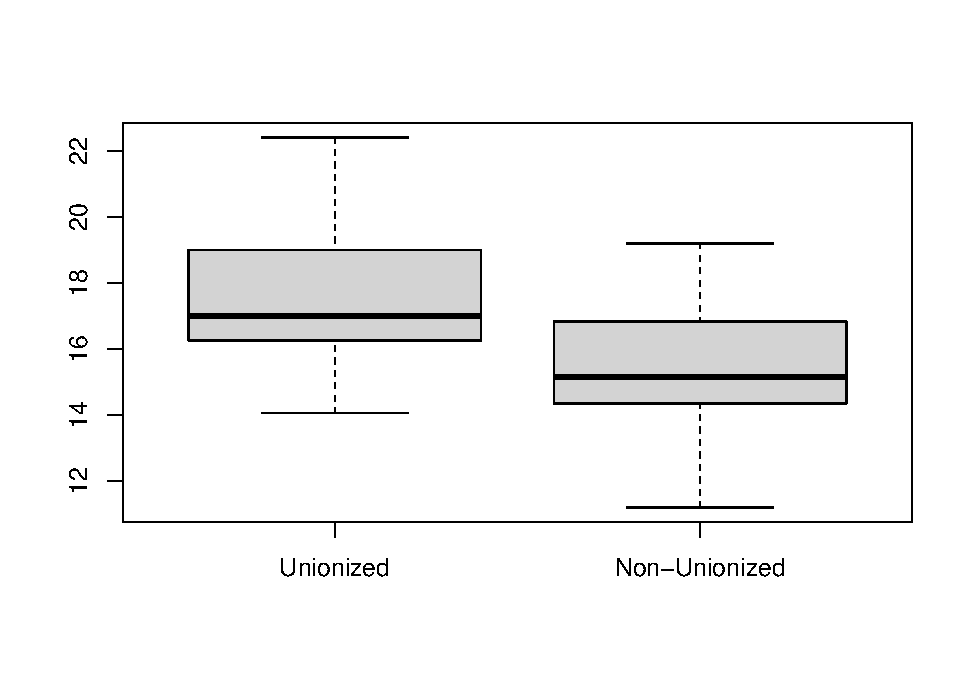
\includegraphics{Estimation-and-Confidence-intervals_files/figure-latex/unnamed-chunk-29-1.pdf}

\begin{Shaded}
\begin{Highlighting}[]
\NormalTok{union\_dat }\OtherTok{\textless{}{-}} \FunctionTok{data.frame}\NormalTok{(}\AttributeTok{wages=}\FunctionTok{c}\NormalTok{(iscritte, non\_iscritte),}\AttributeTok{Union =} \FunctionTok{factor}\NormalTok{(}\FunctionTok{rep}\NormalTok{(}\FunctionTok{c}\NormalTok{(}\StringTok{"Unionized"}\NormalTok{, }\StringTok{"Non{-}Unionized"}\NormalTok{),}\AttributeTok{times=}\FunctionTok{c}\NormalTok{(}\FunctionTok{length}\NormalTok{(iscritte), }\FunctionTok{length}\NormalTok{(non\_iscritte)))))}
\FunctionTok{ggplot}\NormalTok{(union\_dat, }\FunctionTok{aes}\NormalTok{(}\AttributeTok{x =}\NormalTok{ Union, }\AttributeTok{y=}\NormalTok{wages, }\AttributeTok{fill=}\NormalTok{Union))}\SpecialCharTok{+}
  \FunctionTok{geom\_boxplot}\NormalTok{()}
\end{Highlighting}
\end{Shaded}

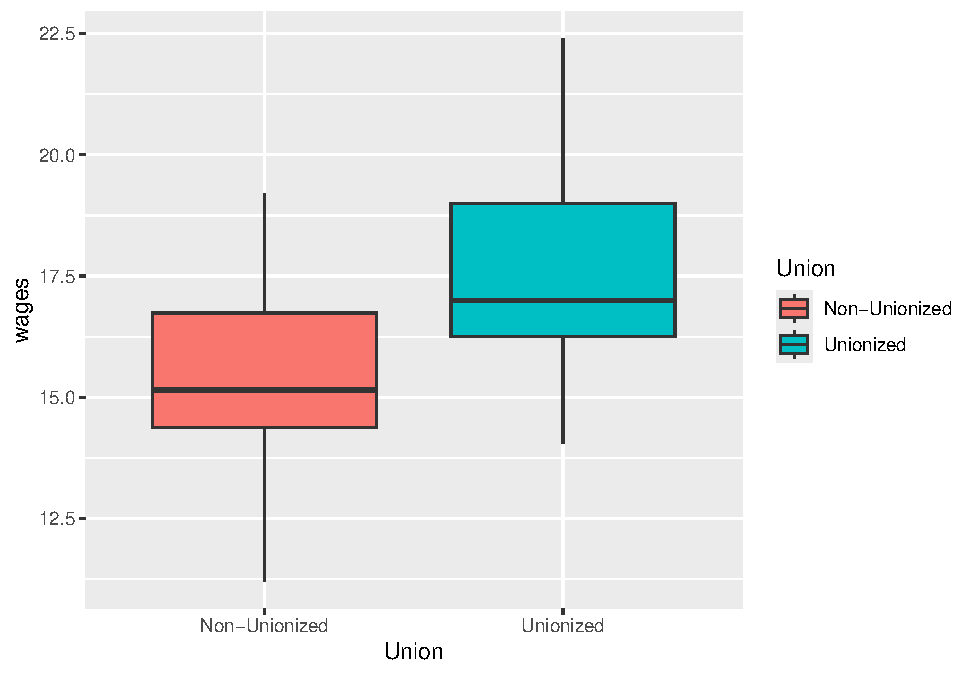
\includegraphics{Estimation-and-Confidence-intervals_files/figure-latex/unnamed-chunk-29-2.pdf}

The boxplot comparison suggests that unionized women earn more on
average than non-unionized women, but this visualization does not
provide any measure of statistical significance or reliability.

Assume that the wages of both groups follow a normal distribution with
means \(\mu_1\) and \(\mu_2\), respectively, and the same variance
\(\sigma_1 = \sigma_2\). We also assume the two populations are
independent. The sample means are:

\begin{Shaded}
\begin{Highlighting}[]
\NormalTok{mu1 }\OtherTok{\textless{}{-}} \FunctionTok{mean}\NormalTok{(iscritte)}
\NormalTok{mu2 }\OtherTok{\textless{}{-}} \FunctionTok{mean}\NormalTok{(non\_iscritte)}
\FunctionTok{c}\NormalTok{(mu1, mu2)}
\end{Highlighting}
\end{Shaded}

\begin{verbatim}
## [1] 17.53667 15.36000
\end{verbatim}

Since we assume equal variances, we calculate the pooled variance:

\begin{Shaded}
\begin{Highlighting}[]
\NormalTok{s1 }\OtherTok{\textless{}{-}} \FunctionTok{var}\NormalTok{(iscritte)}
\NormalTok{s2 }\OtherTok{\textless{}{-}} \FunctionTok{var}\NormalTok{(non\_iscritte)}
\NormalTok{n }\OtherTok{\textless{}{-}} \FunctionTok{length}\NormalTok{(iscritte)}
\NormalTok{m }\OtherTok{\textless{}{-}} \FunctionTok{length}\NormalTok{(non\_iscritte)}
\NormalTok{s }\OtherTok{\textless{}{-}}\NormalTok{ ((n }\SpecialCharTok{{-}} \DecValTok{1}\NormalTok{) }\SpecialCharTok{*}\NormalTok{ s1 }\SpecialCharTok{+}\NormalTok{ (m }\SpecialCharTok{{-}} \DecValTok{1}\NormalTok{) }\SpecialCharTok{*}\NormalTok{ s2) }\SpecialCharTok{/}\NormalTok{ (n }\SpecialCharTok{+}\NormalTok{ m }\SpecialCharTok{{-}} \DecValTok{2}\NormalTok{)}
\end{Highlighting}
\end{Shaded}

We now compute a confidence interval for the difference in means

\begin{Shaded}
\begin{Highlighting}[]
\NormalTok{interval }\OtherTok{\textless{}{-}} \FunctionTok{c}\NormalTok{(}
\NormalTok{  mu1 }\SpecialCharTok{{-}}\NormalTok{ mu2 }\SpecialCharTok{{-}} \FunctionTok{qt}\NormalTok{(}\DecValTok{1} \SpecialCharTok{{-}}\NormalTok{ alpha }\SpecialCharTok{/} \DecValTok{2}\NormalTok{, n }\SpecialCharTok{+}\NormalTok{ m }\SpecialCharTok{{-}} \DecValTok{2}\NormalTok{) }\SpecialCharTok{*} \FunctionTok{sqrt}\NormalTok{(s }\SpecialCharTok{*}\NormalTok{ (}\DecValTok{1} \SpecialCharTok{/}\NormalTok{ n }\SpecialCharTok{+} \DecValTok{1} \SpecialCharTok{/}\NormalTok{ m)),}
\NormalTok{  mu1 }\SpecialCharTok{{-}}\NormalTok{ mu2 }\SpecialCharTok{+} \FunctionTok{qt}\NormalTok{(}\DecValTok{1} \SpecialCharTok{{-}}\NormalTok{ alpha }\SpecialCharTok{/} \DecValTok{2}\NormalTok{, n }\SpecialCharTok{+}\NormalTok{ m }\SpecialCharTok{{-}} \DecValTok{2}\NormalTok{) }\SpecialCharTok{*} \FunctionTok{sqrt}\NormalTok{(s }\SpecialCharTok{*}\NormalTok{ (}\DecValTok{1} \SpecialCharTok{/}\NormalTok{ n }\SpecialCharTok{+} \DecValTok{1} \SpecialCharTok{/}\NormalTok{ m))}
\NormalTok{)}
\NormalTok{interval}
\end{Highlighting}
\end{Shaded}

\begin{verbatim}
## [1] 0.963342 3.389991
\end{verbatim}

\hypertarget{paired-samples}{%
\paragraph{Paired samples}\label{paired-samples}}

Let's now see the last case, i.e., we have a paired sampling design. A
random sample is selected from one population, and each statistical unit
provides two observations. Each pair of observations shares a common
element: the individual on whom the measurements were taken. The two
observations on the same subject are not independent because they are
influenced by common individual factors.

Given \(X_1 \sim N(\mu_1,\sigma^2_1)\) and
\(X_2\sim N(\mu_2,\sigma^2_2)\), when paired sampling is used, we
consider the random variable ``difference'' as:
\[D=X_1-X_2 \sim N(\mu_1-\mu_2,\sigma^2_{X_1-X_2})\].

The parameter of interest in this case becomes the difference of means
\(\mu_D=\mu_1-\mu_2\). We then consider the estimator
\(\bar{D} = \sum_{i=1}^n \frac{X_{1i} - X_{2i}}{n}\). Since also here we
do not know \(\sigma^2_D\), we plug-in the estimator
\[s^2_D = \frac{1}{n-1}\sum_{i=1}^n (D_i-\bar{D})^2.\] Finally the
confidence intervals at level \(1-\alpha\) is computed as
\[IC_{1-\alpha}(\mu_d)=\left[\bar{D}-t_{\alpha/2,n-1}\frac{\sigma_D}{\sqrt{n}},\bar{D}+t_{\alpha/2,n-1}\frac{\sigma_D}{\sqrt{n}}\right]\]
As you can note, this is equal to the confidence interval of the simple
t-test for the mean \(\mu\) but considering the new random variable
\(D\) instead of \(X\).

For example, considering the data set dat previously loaded, we can
compare the Response\_Time collected in occasion 0 and occasion 1. This
data are paired, since they refer to the same observation.

\begin{Shaded}
\begin{Highlighting}[]
\FunctionTok{t.test}\NormalTok{(dat}\SpecialCharTok{$}\NormalTok{Response\_Time[}\FunctionTok{which}\NormalTok{(dat}\SpecialCharTok{$}\NormalTok{Time}\SpecialCharTok{==}\DecValTok{1} \SpecialCharTok{\&}\NormalTok{ dat}\SpecialCharTok{$}\NormalTok{Group}\SpecialCharTok{==}\StringTok{"Control"}\NormalTok{)],}
\NormalTok{       dat}\SpecialCharTok{$}\NormalTok{Response\_Time[}\FunctionTok{which}\NormalTok{(dat}\SpecialCharTok{$}\NormalTok{Time}\SpecialCharTok{==}\DecValTok{2}\SpecialCharTok{\&}\NormalTok{ dat}\SpecialCharTok{$}\NormalTok{Group}\SpecialCharTok{==}\StringTok{"Control"}\NormalTok{)], }
       \AttributeTok{conf.level =} \FloatTok{0.95}\NormalTok{,}
       \AttributeTok{var.equal =} \ConstantTok{FALSE}\NormalTok{,}
       \AttributeTok{paired =} \ConstantTok{TRUE}\NormalTok{)}
\end{Highlighting}
\end{Shaded}

\begin{verbatim}
## 
##  Paired t-test
## 
## data:  dat$Response_Time[which(dat$Time == 1 & dat$Group == "Control")] and dat$Response_Time[which(dat$Time == 2 & dat$Group == "Control")]
## t = -12.353, df = 24, p-value = 6.847e-12
## alternative hypothesis: true mean difference is not equal to 0
## 95 percent confidence interval:
##  -238.4414 -170.1697
## sample estimates:
## mean difference 
##       -204.3055
\end{verbatim}

\end{document}
